\chapter{Theoretical Background}\label{chap:theory}
\begin{chapabstract}

    In this chapter, I put the physical mechanism of radio emissions related to our study.
    At low frequencies, we can observe free-free (Bremsstrahlung) and synchrotron radiations.
    Both emissions are the continuum emissions.
    While the free-free radiation is usually dominant from a galaxy at $30 \sim 200\GHz$, the synchrotron radiation is dominant less than $30\GHz$ (Figure)

\end{chapabstract}



\section{Free-free radiation}

\begin{figure}[htbp]
	\centering
	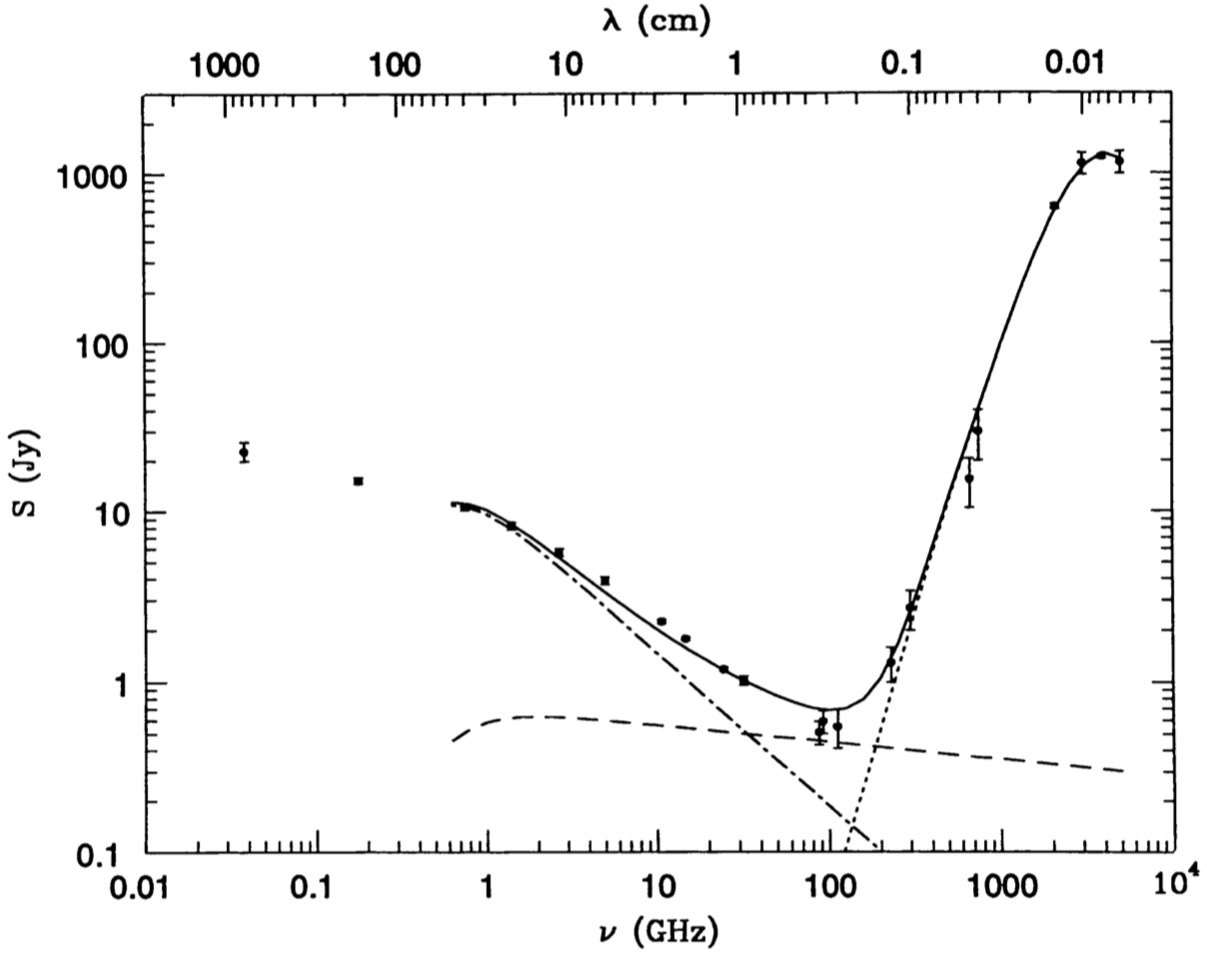
\includegraphics[width=.7\linewidth]{Chapter_2/Figures/Condon1992_Figure1.png}
    \caption[Reprint from \citet{Condon1992a} (Figure~1)]{\label{fig:Condon1992_figure1}
        (Reprint from \citet{Condon1992a}, Figure~1)\\
        This figure shows the spectral energy distribution of M82.
        The dotted line shows the dust thermal emission which is dominant at higher than $200\GHz$.
        The dashed line shows the free-free radiation from the \ih~regions around massive stars,which is dominant at $30 \sim 200\GHz$.
        The dot-dash line shows the synchrotron radiation emitted by the high energy electrons, which is dominant at less than $30\GHz$.
    }
\end{figure}




















\section{Synchrotron radiation}
